\documentclass{standalone}
\usepackage{tikz}
\usetikzlibrary{patterns, positioning}


\begin{document}
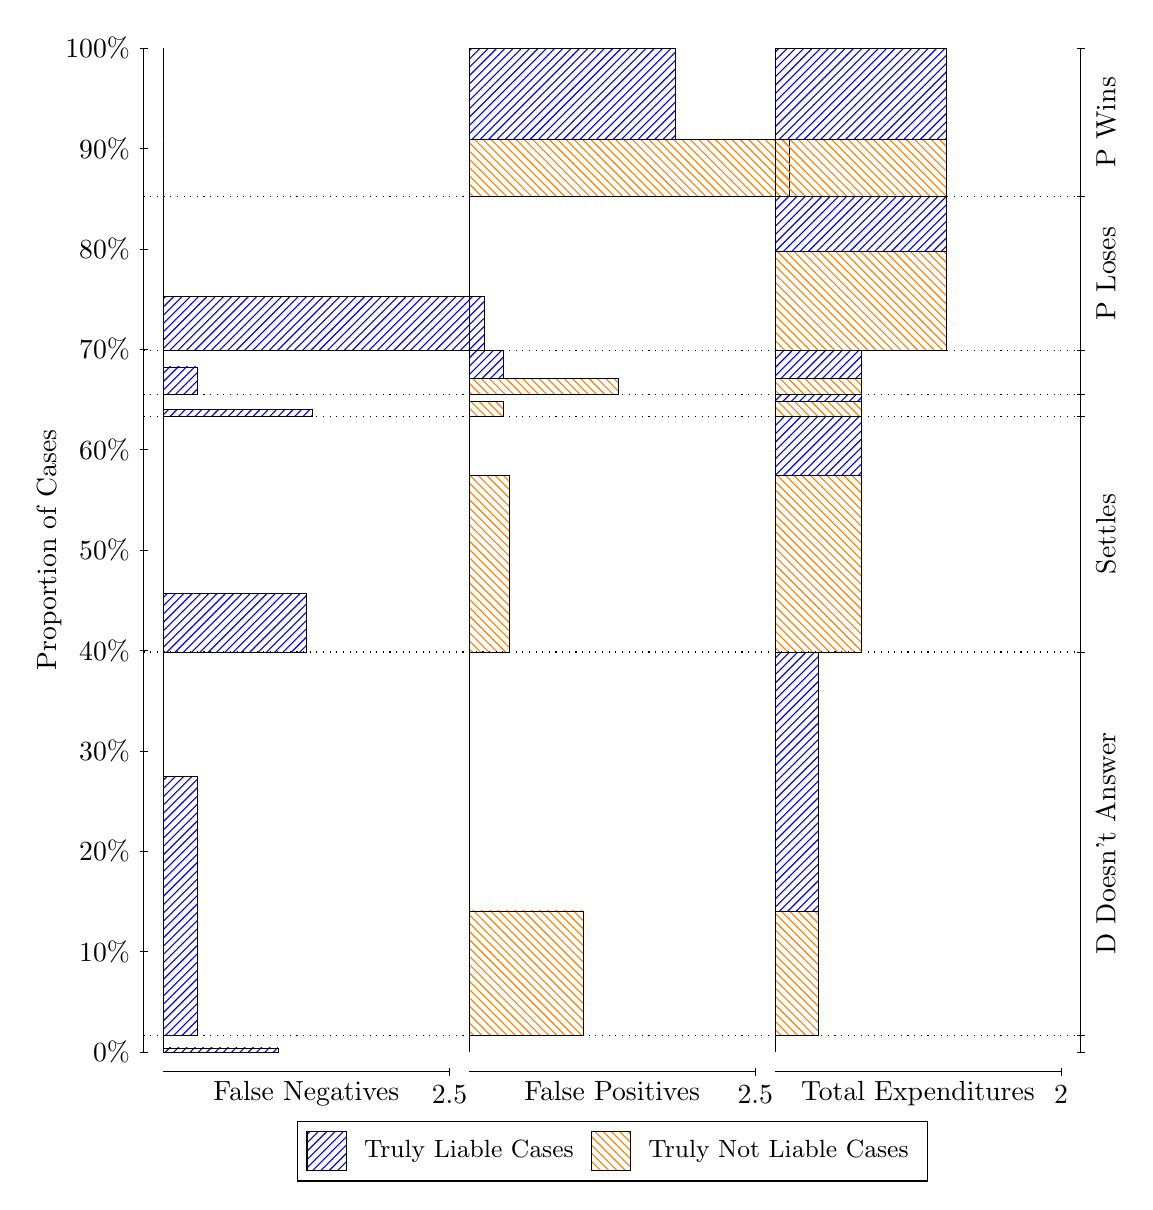
\begin{tikzpicture}
\draw[black, very thin] (1.5,1.75) -- (1.5,14.5);
\node[rotate=90, text=black, anchor=center] at (0.3, 8.125) {Proportion of Cases};
\draw[black, very thin] (1.45,1.75) -- (1.55,1.75);
\node[text=black, anchor=east] at (1.45, 1.75) {0\%};
\draw[black, very thin] (1.45,3.025) -- (1.55,3.025);
\node[text=black, anchor=east] at (1.45, 3.025) {10\%};
\draw[black, very thin] (1.45,4.3) -- (1.55,4.3);
\node[text=black, anchor=east] at (1.45, 4.3) {20\%};
\draw[black, very thin] (1.45,5.575) -- (1.55,5.575);
\node[text=black, anchor=east] at (1.45, 5.575) {30\%};
\draw[black, very thin] (1.45,6.85) -- (1.55,6.85);
\node[text=black, anchor=east] at (1.45, 6.85) {40\%};
\draw[black, very thin] (1.45,8.125) -- (1.55,8.125);
\node[text=black, anchor=east] at (1.45, 8.125) {50\%};
\draw[black, very thin] (1.45,9.4) -- (1.55,9.4);
\node[text=black, anchor=east] at (1.45, 9.4) {60\%};
\draw[black, very thin] (1.45,10.675) -- (1.55,10.675);
\node[text=black, anchor=east] at (1.45, 10.675) {70\%};
\draw[black, very thin] (1.45,11.95) -- (1.55,11.95);
\node[text=black, anchor=east] at (1.45, 11.95) {80\%};
\draw[black, very thin] (1.45,13.225) -- (1.55,13.225);
\node[text=black, anchor=east] at (1.45, 13.225) {90\%};
\draw[black, very thin] (1.45,14.5) -- (1.55,14.5);
\node[text=black, anchor=east] at (1.45, 14.5) {100\%};

\draw[black, very thin] (13.4,1.75) -- (13.4,14.5);
\draw[black, very thin] (13.35,1.75) -- (13.45,1.75);
\node[anchor=west] at (13.35, 1.75) {};
\draw[black, very thin] (13.35,1.9648) -- (13.45,1.9648);
\node[anchor=west] at (13.35, 1.9648) {};
\draw[black, very thin] (13.35,6.8294) -- (13.45,6.8294);
\node[anchor=west] at (13.35, 6.8294) {};
\draw[black, very thin] (13.35,9.8252) -- (13.45,9.8252);
\node[anchor=west] at (13.35, 9.8252) {};
\draw[black, very thin] (13.35,10.102) -- (13.45,10.102);
\node[anchor=west] at (13.35, 10.102) {};
\draw[black, very thin] (13.35,10.657) -- (13.45,10.657);
\node[anchor=west] at (13.35, 10.657) {};
\draw[black, very thin] (13.35,12.614) -- (13.45,12.614);
\node[anchor=west] at (13.35, 12.614) {};
\draw[black, very thin] (13.35,14.5) -- (13.45,14.5);
\node[anchor=west] at (13.35, 14.5) {};

\draw[black, very thin, pattern color=blue, pattern=north east lines] (1.75,1.75) rectangle (3.2033,1.8027);
\draw[black, very thin, pattern color=orange, pattern=north west lines] (1.75,1.8027) rectangle (1.75,1.9648);
\draw[black, very thin, pattern color=blue, pattern=north east lines] (1.75,1.9648) rectangle (2.186,5.2527);
\draw[black, very thin, pattern color=orange, pattern=north west lines] (1.75,5.2527) rectangle (1.75,6.8294);
\draw[black, very thin, pattern color=blue, pattern=north east lines] (1.75,6.8294) rectangle (3.5667,7.5781);
\draw[black, very thin, pattern color=orange, pattern=north west lines] (1.75,7.5781) rectangle (1.75,9.8252);
\draw[black, very thin, pattern color=blue, pattern=north east lines] (1.75,9.8252) rectangle (3.6393,9.9106);
\draw[black, very thin, pattern color=orange, pattern=north west lines] (1.75,9.9106) rectangle (1.75,10.102);
\draw[black, very thin, pattern color=blue, pattern=north east lines] (1.75,10.102) rectangle (2.186,10.451);
\draw[black, very thin, pattern color=orange, pattern=north west lines] (1.75,10.451) rectangle (1.75,10.657);
\draw[black, very thin, pattern color=blue, pattern=north east lines] (1.75,10.657) rectangle (5.8193,11.349);
\draw[black, very thin, pattern color=orange, pattern=north west lines] (1.75,11.349) rectangle (1.75,12.614);
\draw[black, very thin, pattern color=orange, pattern=north west lines] (1.75,12.614) rectangle (1.75,13.34);
\draw[black, very thin, pattern color=blue, pattern=north east lines] (1.75,13.34) rectangle (1.75,14.5);
\draw[black, very thin, pattern color=orange, pattern=north west lines] (5.6333,1.75) rectangle (5.6333,1.9121);
\draw[black, very thin, pattern color=blue, pattern=north east lines] (5.6333,1.9121) rectangle (5.6333,1.9648);
\draw[black, very thin, pattern color=orange, pattern=north west lines] (5.6333,1.9648) rectangle (7.0867,3.5415);
\draw[black, very thin, pattern color=blue, pattern=north east lines] (5.6333,3.5415) rectangle (5.6333,6.8294);
\draw[black, very thin, pattern color=orange, pattern=north west lines] (5.6333,6.8294) rectangle (6.142,9.0766);
\draw[black, very thin, pattern color=blue, pattern=north east lines] (5.6333,9.0766) rectangle (5.6333,9.8252);
\draw[black, very thin, pattern color=orange, pattern=north west lines] (5.6333,9.8252) rectangle (6.0693,10.017);
\draw[black, very thin, pattern color=blue, pattern=north east lines] (5.6333,10.017) rectangle (5.6333,10.102);
\draw[black, very thin, pattern color=orange, pattern=north west lines] (5.6333,10.102) rectangle (7.5227,10.309);
\draw[black, very thin, pattern color=blue, pattern=north east lines] (5.6333,10.309) rectangle (6.0693,10.657);
\draw[black, very thin, pattern color=orange, pattern=north west lines] (5.6333,10.657) rectangle (5.6333,11.922);
\draw[black, very thin, pattern color=blue, pattern=north east lines] (5.6333,11.922) rectangle (5.6333,12.614);
\draw[black, very thin, pattern color=orange, pattern=north west lines] (5.6333,12.614) rectangle (9.7027,13.34);
\draw[black, very thin, pattern color=blue, pattern=north east lines] (5.6333,13.34) rectangle (8.2493,14.5);
\draw[black, very thin, pattern color=orange, pattern=north west lines] (9.5167,1.75) rectangle (9.5167,1.9121);
\draw[black, very thin, pattern color=blue, pattern=north east lines] (9.5167,1.9121) rectangle (9.5167,1.9648);
\draw[black, very thin, pattern color=orange, pattern=north west lines] (9.5167,1.9648) rectangle (10.062,3.5415);
\draw[black, very thin, pattern color=blue, pattern=north east lines] (9.5167,3.5415) rectangle (10.062,6.8294);
\draw[black, very thin, pattern color=orange, pattern=north west lines] (9.5167,6.8294) rectangle (10.607,9.0766);
\draw[black, very thin, pattern color=blue, pattern=north east lines] (9.5167,9.0766) rectangle (10.607,9.8252);
\draw[black, very thin, pattern color=orange, pattern=north west lines] (9.5167,9.8252) rectangle (10.607,10.017);
\draw[black, very thin, pattern color=blue, pattern=north east lines] (9.5167,10.017) rectangle (10.607,10.102);
\draw[black, very thin, pattern color=orange, pattern=north west lines] (9.5167,10.102) rectangle (10.607,10.309);
\draw[black, very thin, pattern color=blue, pattern=north east lines] (9.5167,10.309) rectangle (10.607,10.657);
\draw[black, very thin, pattern color=orange, pattern=north west lines] (9.5167,10.657) rectangle (11.697,11.922);
\draw[black, very thin, pattern color=blue, pattern=north east lines] (9.5167,11.922) rectangle (11.697,12.614);
\draw[black, very thin, pattern color=orange, pattern=north west lines] (9.5167,12.614) rectangle (11.697,13.34);
\draw[black, very thin, pattern color=blue, pattern=north east lines] (9.5167,13.34) rectangle (11.697,14.5);
\draw[black, dotted] (1.5,1.9648) -- (13.4,1.9648);
\draw[black, dotted] (1.5,6.8294) -- (13.4,6.8294);
\draw[black, dotted] (1.5,9.8252) -- (13.4,9.8252);
\draw[black, dotted] (1.5,10.102) -- (13.4,10.102);
\draw[black, dotted] (1.5,10.657) -- (13.4,10.657);
\draw[black, dotted] (1.5,12.614) -- (13.4,12.614);
\draw[black, very thin] (1.75,1.5) -- (5.3833,1.5);
\node[text=black, anchor=north] at (3.5667, 1.5) {False Negatives};
\draw[black, very thin] (5.3833,1.45) -- (5.3833,1.55);
\node[text=black, anchor=north] at (5.3833, 1.45) {2.5};

\draw[black, very thin] (5.6333,1.5) -- (9.2667,1.5);
\node[text=black, anchor=north] at (7.45, 1.5) {False Positives};
\draw[black, very thin] (9.2667,1.45) -- (9.2667,1.55);
\node[text=black, anchor=north] at (9.2667, 1.45) {2.5};

\draw[black, very thin] (9.5167,1.5) -- (13.15,1.5);
\node[text=black, anchor=north] at (11.333, 1.5) {Total Expenditures};
\draw[black, very thin] (13.15,1.45) -- (13.15,1.55);
\node[text=black, anchor=north] at (13.15, 1.45) {2};


\node[text=black, centered, rotate=90] at (13.72, 4.3971) {D Doesn't Answer};
\node[text=black, centered, rotate=90] at (13.72, 8.3273) {Settles};


\node[text=black, centered, rotate=90] at (13.72, 11.636) {P Loses};
\node[text=black, centered, rotate=90] at (13.72, 13.557) {P Wins};

\draw (7.449999999999999,1.5) node[draw=none] (baseCoordinate) {};
\begin{scope}[align=center]
        \matrix[scale=0.5, draw=black, below=0.5cm of baseCoordinate, nodes={draw}, column sep=0.1cm]{
            \node[rectangle, draw, minimum width=0.5cm, minimum height=0.5cm, pattern color=blue, pattern=north east lines] {}; &
            \node[draw=none, font=\small, text=black] (B) {Truly Liable Cases}; &
            \node[rectangle, draw, minimum width=0.5cm, minimum height=0.5cm, pattern color=orange, pattern=north west lines] {}; &
            \node[draw=none, font=\small, text=black] (B) {Truly Not Liable Cases}; \\
            };
\end{scope}

\end{tikzpicture}
\end{document}